\newcommand{\placetextbox}[3]{% \placetextbox{<horizontal pos>}{<vertical pos>}{<stuff>}
	\setbox0=\hbox{#3}% Put <stuff> in a box
	\AddToShipoutPictureFG*{% Add <stuff> to current page foreground
		\put(\LenToUnit{#1\paperwidth},\LenToUnit{#2\paperheight}){\vtop{{\null}\makebox[0pt][c]{#3}}}%
	}%
}%

\pagenumbering{gobble}
\fancyhf{}                          % Очищаем текущие значения

\chapter{Выполнение лабораторной работы}						

%\placetextbox{0.55}{0.1}{\Huge \textit{This is my text qweqwqweqw.}}%
%  {<width>}
%  [<left handle>,<top handle>]
%  (<leftmargin>,<topmargin>)

\begin{textblock}{10}[0,0](4.5, 10.9)
	\begin{center}
		\Large	Лабораторная работа № 3\\
	\end{center}
\end{textblock}

\begin{textblock}{5}[0,0](5, 11.5)
\begin{center}
\large	Распараллеливание алгоритма с помощью библиотеки CCR\\
\end{center}
\end{textblock}

\begin{textblock}{3}[0,0](12.5, 11.75)
	\pageref{LastPage}
\end{textblock}

\begin{textblock}{3}[0,0](11, 12.3)
	14-В-2
\end{textblock}
	
\section{Цель и вариант задания на лабораторную работу}	
	Целью данной лабораторной работы является получение представления о возможностях библиотеки Corrent and Coordination Runtime для организации параллельных вычислений.
	
	Вариант индивидуального задания:
	
	 Разработать алгоритм скалярного произведения n-мерных векторов

\section{Библиотека Concurrent and Coordination Runtime}
Библиотека Concurrent and Coordination Runtime (CCR) предназначена
для организации обработки данных с помощью параллельно и асинхронно
выполняющихся методов. Взаимодействие между такими методами
организуется на основе сообщений. Рассылка сообщений основана на
использовании портов.

Основные понятия CCR:

1) сообщение – экземпляр любого типа данных;

2) порт – очередь сообщений типа FIFO,
сообщение остаётся в порте пока не будут извлечено из очереди порта
получателем.
Отправка сообщения в порт:
p.Post(1);

3) получатель – структура, которая выполняет обработку сообщений.

Данная структура объединяет:

а) один или несколько портов, в которые отправляются сообщения;

б) методы, которые используются для обработки
сообщений;

в) логическое условие, определяющее ситуации, в которых
активизируется тот или иной получатель.

Получатели сообщений бывают двух типов: временные и постоянные. Временный получатель, обработав
сообщение, удаляется из списка получателей
сообщений данного порта.

4) процессом запуска задач управляет диспетчер. После выполнения
условий активации задачи (получение портом сообщения) диспетчер назначает задаче поток из пула
потоков, в котором она будет выполняться.

\chapter{Выполнение лабораторной работы}						

\pagenumbering{arabic}
\setcounter{page}{3}
\rfoot{\thepage}
\fancyfootoffset[L]{-6cm}
\setlength{\footskip}{1.3cm}
\cfoot[EO]{\fontsize{16}{12} \selectfont \textit{Лабораторная работа № 3} }

\section{Объявление структур данных}

Развмерность умножаемых векторов, количество компонент векторов, обрабатываемых в одном потоке, вектора a и b и переменные для хранения результата определены глобально:
\begin{figure}[h!]
	\center{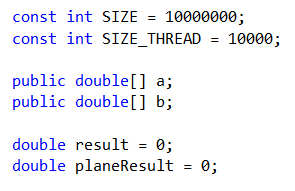
\includegraphics[scale = 0.5]{glob.png}}
\end{figure}

В методе Start() запускаются вычисления. Сначала в методе
выполняется вычисление скалярного скалярного произведения n-мерных векторов последовательным алгоритмом, затем та же задача решается с помощью
параллельных вычислений. Рассмотрим этот метод:
Выполняется инициализация структур данных:
\begin{figure}[h!]
	\center{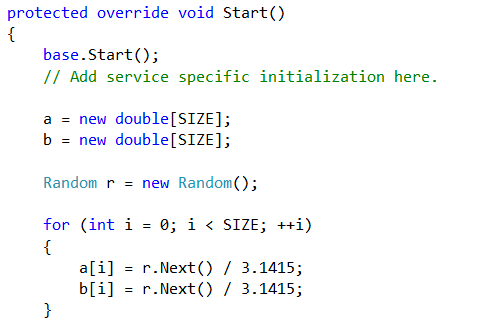
\includegraphics[scale = 0.5]{start.png}}
\end{figure}

\section{Последовательный алгоритм вычисления скалярного произведения n-мерных векторов }

 
 \begin{figure}[h!]
 	\center{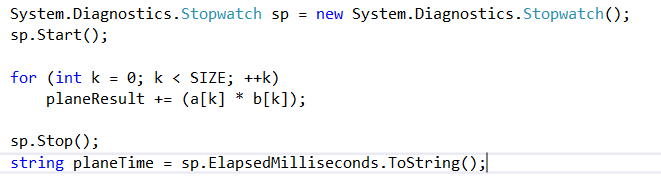
\includegraphics[scale = 0.5]{seq.png}}
 \end{figure}
 
\clearpage

\section{Параллельный алгоритм вычисления скалярного произведения n-мерных векторов}

Параллельная обработка выполняется с помощью запуска нескольких
копий вычислительного метода. Каждая копия метода выполняет
обработку определённой части исходных данных. Для описания задания
для каждого метода используется класс InputData:

\center{public double[] a;\\
public double[] b;\\}
Поле а класса хранит компоненты векторов. Поля рассчитываются с помощью экземпляра вычислительного
метода.

\begin{figure}[h!]
	\center{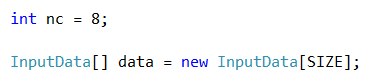
\includegraphics[scale = 0.5]{param.png}}
\end{figure}

Далее, задаются исходные данные для каждого экземпляра
вычислительного метода:

\begin{figure}[h!]
	\center{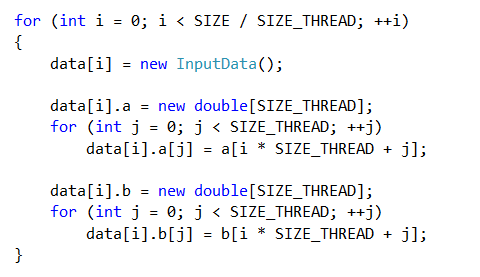
\includegraphics[scale = 0.5]{is_data.png}}
\end{figure}

Создаётся диспетчер с пулом из 8 потоков и описывается порт, в который каждый экземпляр метода Sort() отправляет сообщение после завершения вычислений:

\begin{figure}[h!]
	\center{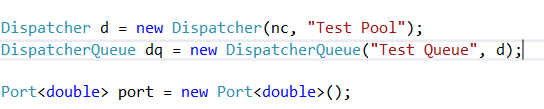
\includegraphics[scale = 0.5]{disp.png}}
\end{figure}

Метод Arbiter.Activate помещает задачи в очередь диспетчера:

\begin{figure}[h!]
	\center{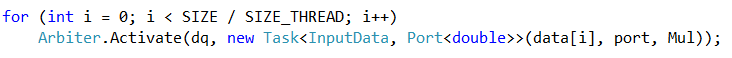
\includegraphics[scale = 0.5]{arb.png}}
\end{figure}

Первый параметр метода Arbiter.Activate – очередь диспетчера,
который будет управлять выполнением задачи, второй параметр –
запускаемая задача.

С помощью метода Arbiter.MultipleItemReceive запускается задача
(приёмник), которая обрабатывает сообщения:

\begin{figure}[h!]
	\center{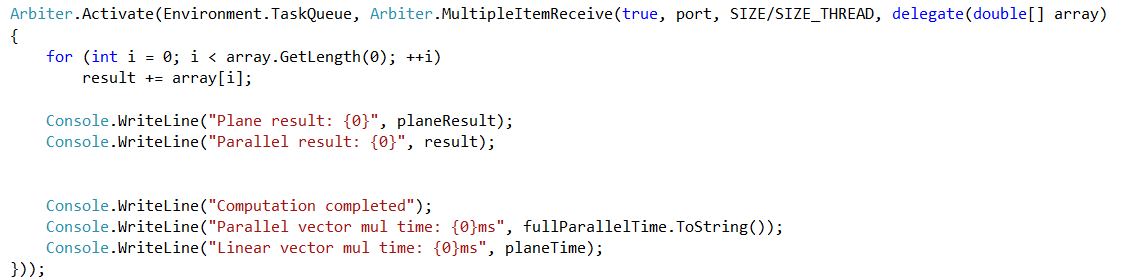
\includegraphics[scale = 0.5]{act.png}}
\end{figure}

Приёмник используется для определения момента окончания
вычислений. Он сработает только после того, как в порт p придут все сообщения. В делегат, описанный в приёмнике,  включим действия,
которые будут выполнены после завершения процесса сортировки в каждом из потоков. Такими действиями является вывод результата, а также подсчет результатов интегрирования подотрезков.

Метод Mul() выполняет скалярное произведение:

\begin{figure}[h!]
	\center{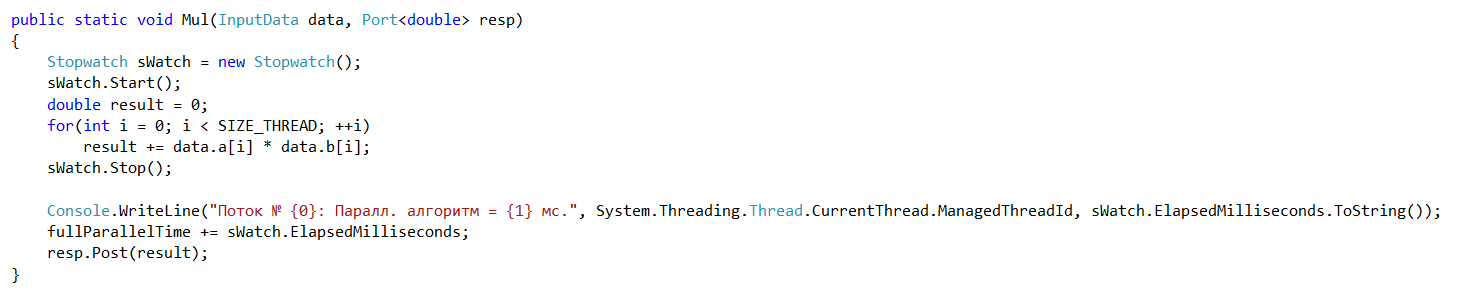
\includegraphics[scale = 0.5]{mul.png}}
\end{figure}

Метод Mul() имеет два параметра:
1) индекс, хранящий значение элемента массива, который определяет
параметры, передаваемые на вход метода;
2) порт завершения, в который отправляется экземпляр класса double после
завершения вычислений.
После завершения вычислений метод Mul отправляет в порт p
значение экземпляра класса double, который необходим определения времени завершения вычислений.
Результат вычислений показан на рисунке:

\begin{figure}[h!]
	\center{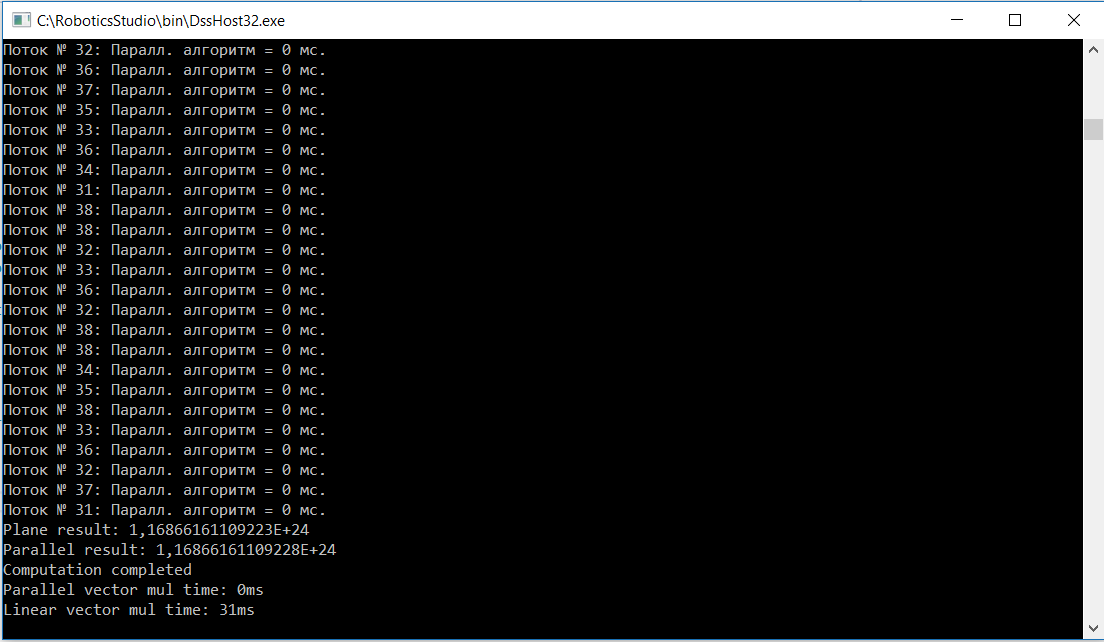
\includegraphics[scale = 0.3]{scr.png}}
\end{figure}


\section*{Выводы}
Таким образом, в ходе данной лабораторной работы были изучены и освоены на практике возможности библиотеки Corrent and Coordination Runtime для организации параллельных вычислений. Разработаны последовательный и параллельный алгоритмы вычисления скалярного произведения n-мерных векторов. Исходя из работы программы можно сделать вывод о том, что время выполнения последовательного алгоритма примерно в несколько раз больше, чем время выполнения параллельного алгоритма, также результаты при последовательном и параллельном алгоритмах одинаковые, то есть программа работает правильно.
\end{document}

